\hypertarget{report-user}{%
\subsection{Report User}\label{report-user}}

\hypertarget{ux3c0ux3b5ux3c1ux3b9ux3b3ux3c1ux3b1ux3c6ux3ae}{%
\subsubsection{Περιγραφή}\label{ux3c0ux3b5ux3c1ux3b9ux3b3ux3c1ux3b1ux3c6ux3ae}}

Ο χρήστης επιθυμεί να αναφέρει έναν άλλο χρήστη της εφαρμογής για
παράνομη ή ανεπιθύμητη δραστηριότητα.

\hypertarget{ux3b2ux3b1ux3c3ux3b9ux3baux3ae-ux3c1ux3bfux3ae}{%
\paragraph{Βασική
Ροή}\label{ux3b2ux3b1ux3c3ux3b9ux3baux3ae-ux3c1ux3bfux3ae}}

\begin{enumerate}
\def\labelenumi{\arabic{enumi}.}
\tightlist
\item
  Ο χρήστης επιλέγει ``Report'' στην οθόνη User Details.
\item
  Το σύστημα εμφανίζει την φόρμα αναφοράς στην οθόνη Report User.
\item
  Ο χρήστης επιλέγει τον λόγο αναφοράς και προσθέτει σχόλια στην οθόνη
  Report User.
\item
  Το σύστημα εμφανίζει τον διάλογο επιβεβαίωσης αναφοράς.
\item
  Ο χρήστης επιλέγει ``Confirm'' στον διάλογο επιβεβαίωσης αναφοράς.
\item
  Το σύστημα δημιουργεί την αναφορά.
\item
  Το σύστημα καταχωρεί την αναφορά στο αρχείο.
\item
  Το σύστημα επεξεργάζεται την αναφορά.
\item
  Το σύστημα αναθέτει ποινή στον αναφερόμενο.
\item
  Το σύστημα εμφανίζει μήνυμα επιτυχίας στην οθόνη User Details.
\end{enumerate}

\hypertarget{ux3b5ux3bdux3b1ux3bbux3bbux3b1ux3baux3c4ux3b9ux3baux3ae-ux3c1ux3bfux3ae-ux3b1ux3c0ux3ccux3c1ux3c1ux3b9ux3c8ux3b7-ux3b1ux3bdux3b1ux3c6ux3bfux3c1ux3acux3c2}{%
\paragraph{Εναλλακτική Ροή: Απόρριψη
Αναφοράς}\label{ux3b5ux3bdux3b1ux3bbux3bbux3b1ux3baux3c4ux3b9ux3baux3ae-ux3c1ux3bfux3ae-ux3b1ux3c0ux3ccux3c1ux3c1ux3b9ux3c8ux3b7-ux3b1ux3bdux3b1ux3c6ux3bfux3c1ux3acux3c2}}

\begin{enumerate}
\def\labelenumi{\arabic{enumi}.}
\setcounter{enumi}{8}
\tightlist
\item
  Το σύστημα απορρίπτει την αναφορά.
\item
  Το σύστημα εμφανίζει μήνυμα επιτυχίας.
\item
  Επιστροφή στην οθόνη User Details.
\end{enumerate}

\hypertarget{ux3b5ux3bdux3b1ux3bbux3bbux3b1ux3baux3c4ux3b9ux3baux3ae-ux3c1ux3bfux3ae-ux3b1ux3baux3cdux3c1ux3c9ux3c3ux3b7}{%
\paragraph{Εναλλακτική Ροή:
Ακύρωση}\label{ux3b5ux3bdux3b1ux3bbux3bbux3b1ux3baux3c4ux3b9ux3baux3ae-ux3c1ux3bfux3ae-ux3b1ux3baux3cdux3c1ux3c9ux3c3ux3b7}}

\begin{enumerate}
\def\labelenumi{\arabic{enumi}.}
\setcounter{enumi}{4}
\tightlist
\item
  Ο χρήστης επιλέγει ``Cancel'' στον διάλογο επιβεβαίωσης αναφοράς.
\item
  Το σύστημα επιστρέφει στην οθόνη Report User.
\end{enumerate}

\hypertarget{ux3b1ux3bdux3acux3bbux3c5ux3c3ux3b7-ux3b5ux3c5ux3c1ux3c9ux3c3ux3c4ux3afux3b1ux3c2}{%
\subsubsection{Ανάλυση
Ευρωστίας}\label{ux3b1ux3bdux3acux3bbux3c5ux3c3ux3b7-ux3b5ux3c5ux3c1ux3c9ux3c3ux3c4ux3afux3b1ux3c2}}

\begin{figure}
\centering
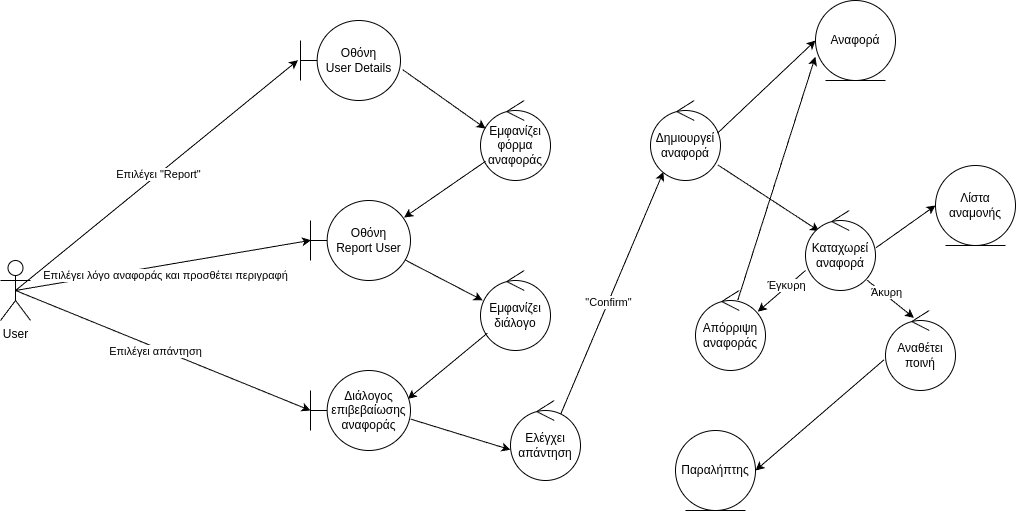
\includegraphics{./report-user-robustness.drawio.png}
\caption{image}
\end{figure}
